\section{Axion search mode}

The motivation to search for the existence of axion dark matter rests in its capability to solve the strong CP-problem. %
In a storage ring environment it could be probed by polarized beams. One looks for a resonance between the natural spin precession in the ring and the oscillating axion field. %
The former is being scanned in the frequency range corresponding to a mass range of interest. Only so-called light axions or axion-like particles (ALPs) , with masses below 0.1 $\mu$eV/c$^2$, %
could be probed in an accelerator, due to the upper limit on the natural spin precession frequency. %
Ultralight axions could be reached by employing spin freezing technologies such as the strictly or quasi frozen spin, spin transparency induced by Siberian snakes, or the Figure-8 ring.~\cite{Filatov:2022lxd}

The pilot experiment to search for axions has been carried out at COSY in 2019.~\cite{JEDI:2022hxa} That experiment achieved an upper limit on the axion-induced EDM approaching $d\,=\,5\cdot 10^{-23}\,e\cdot$cm. The concept of that experiment consists in observing a difference between the vertical projections of the beam's polarization before and after a resonance crossing. Simple statistical considerations~\cite{Aksentev:2026_edm_estimates} show that for that machine the achieved precision is close to the statistical limit. Further improvements could be made by reducing the uncertainty of polarimetry or by lowering the scan speed. The former would lower the observation significance threshold, the latter allow for a greater accumulation of the signal difference. Figure~\ref{fig:Aksentev:Estimates2026:Fig4} presents the possible improvement on the EDM estimate's upper bound. The relationship presented in the figure can be formally expressed by
\begin{equation}\label{eq:Aksentev:Estimates2026:Main}
	\Theta = 2\xi\sqrt{\dot f},
\end{equation}
in which $\xi$ is the significance threshold, $\dot f$ the scan speed, $\Theta$ reflects the axion spin-driving force. The latter quantity converts into the oscillating EDM or the axion wind coupling strength, depending on the theory.

\begin{figure}[h]\centering
	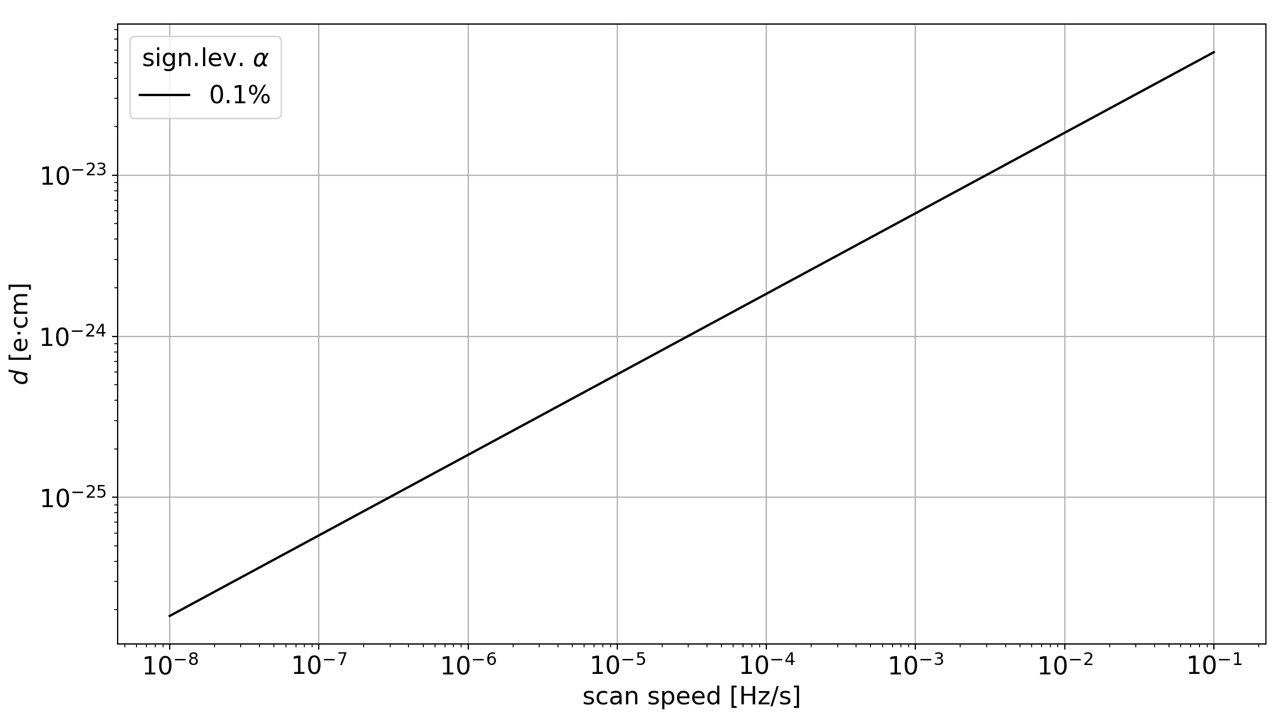
\includegraphics[width=\linewidth]{signal_vs_scan_speed}
	\caption{EDM estimate projection for the pilot experiment.
		\label{fig:Aksentev:Estimates2026:Fig4}
	}
\end{figure}
